\subsection{Dagensløsning}
\subsubsection{Beskrivelse av dagens løsning}

Dagens løsning består av en skinnekonstruksjon boltet til gulvet i hengeren, og en ramme på seks hjul som ruller på denne skinnen. Se Figur \ref{F1} 
\begin{figure}[h!]
\centering   
\subfloat[Rammen]{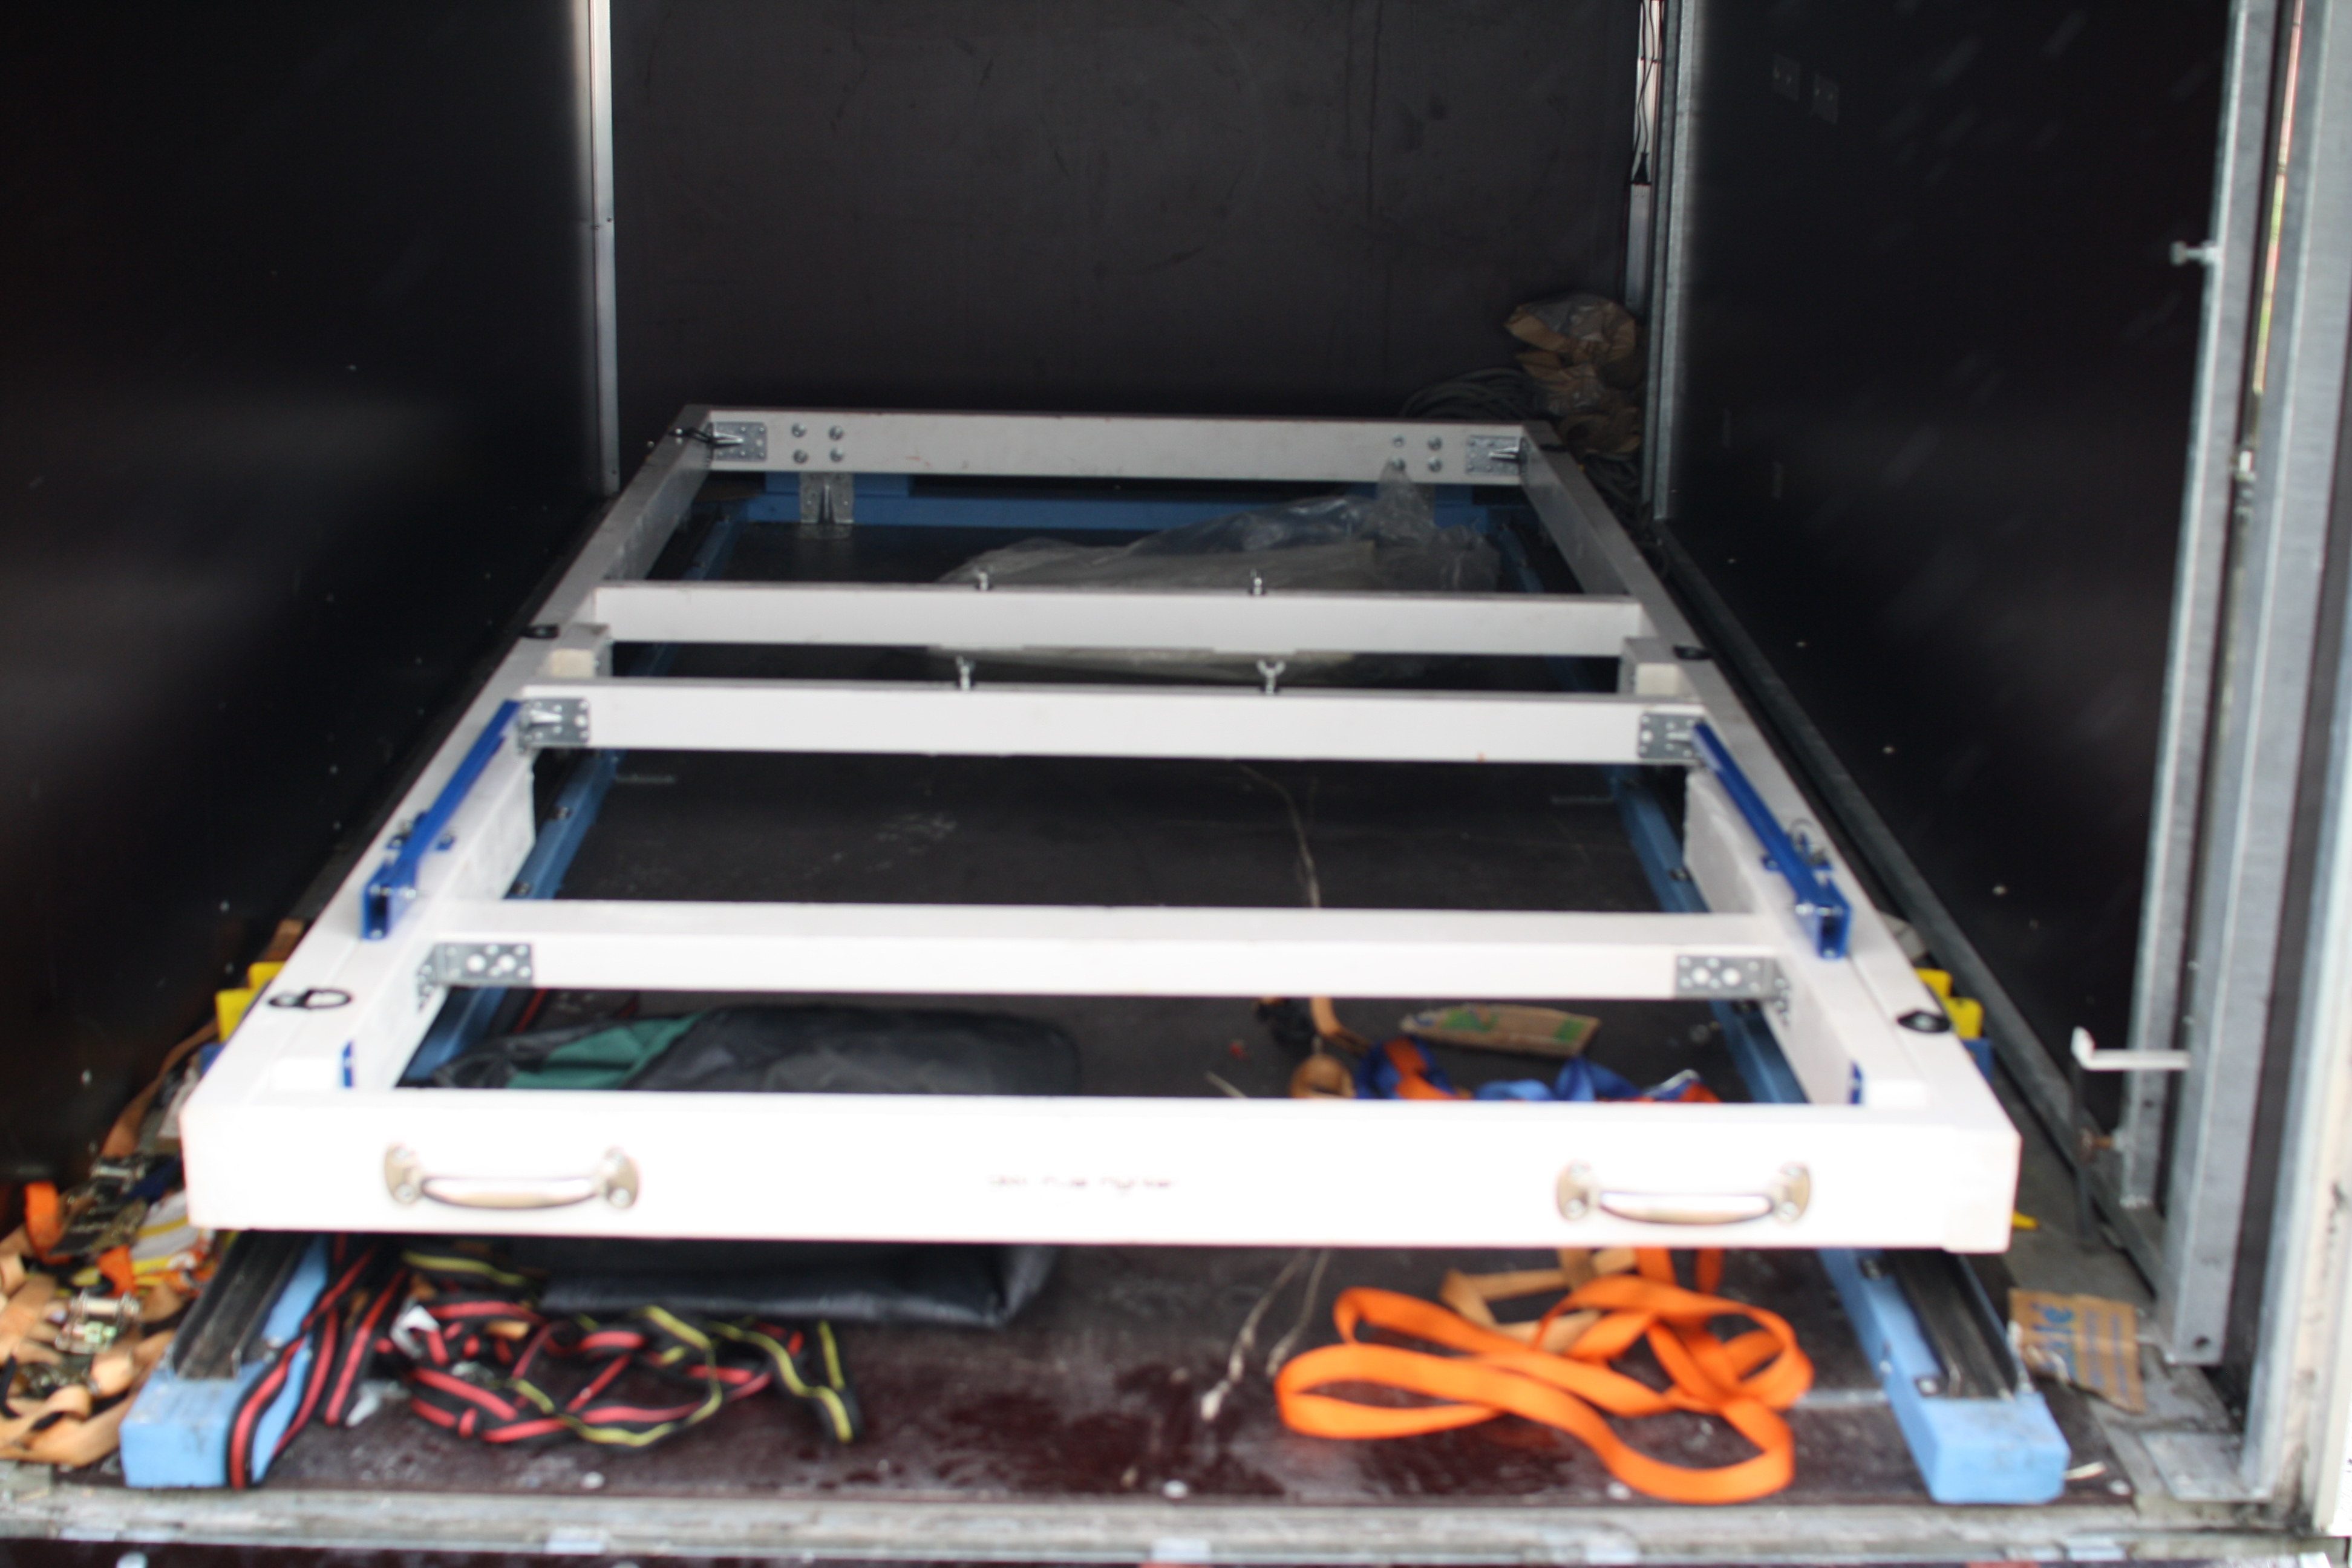
\includegraphics[width=0.5\textwidth]{images/DL1.JPG}}
\subfloat[Hjul]{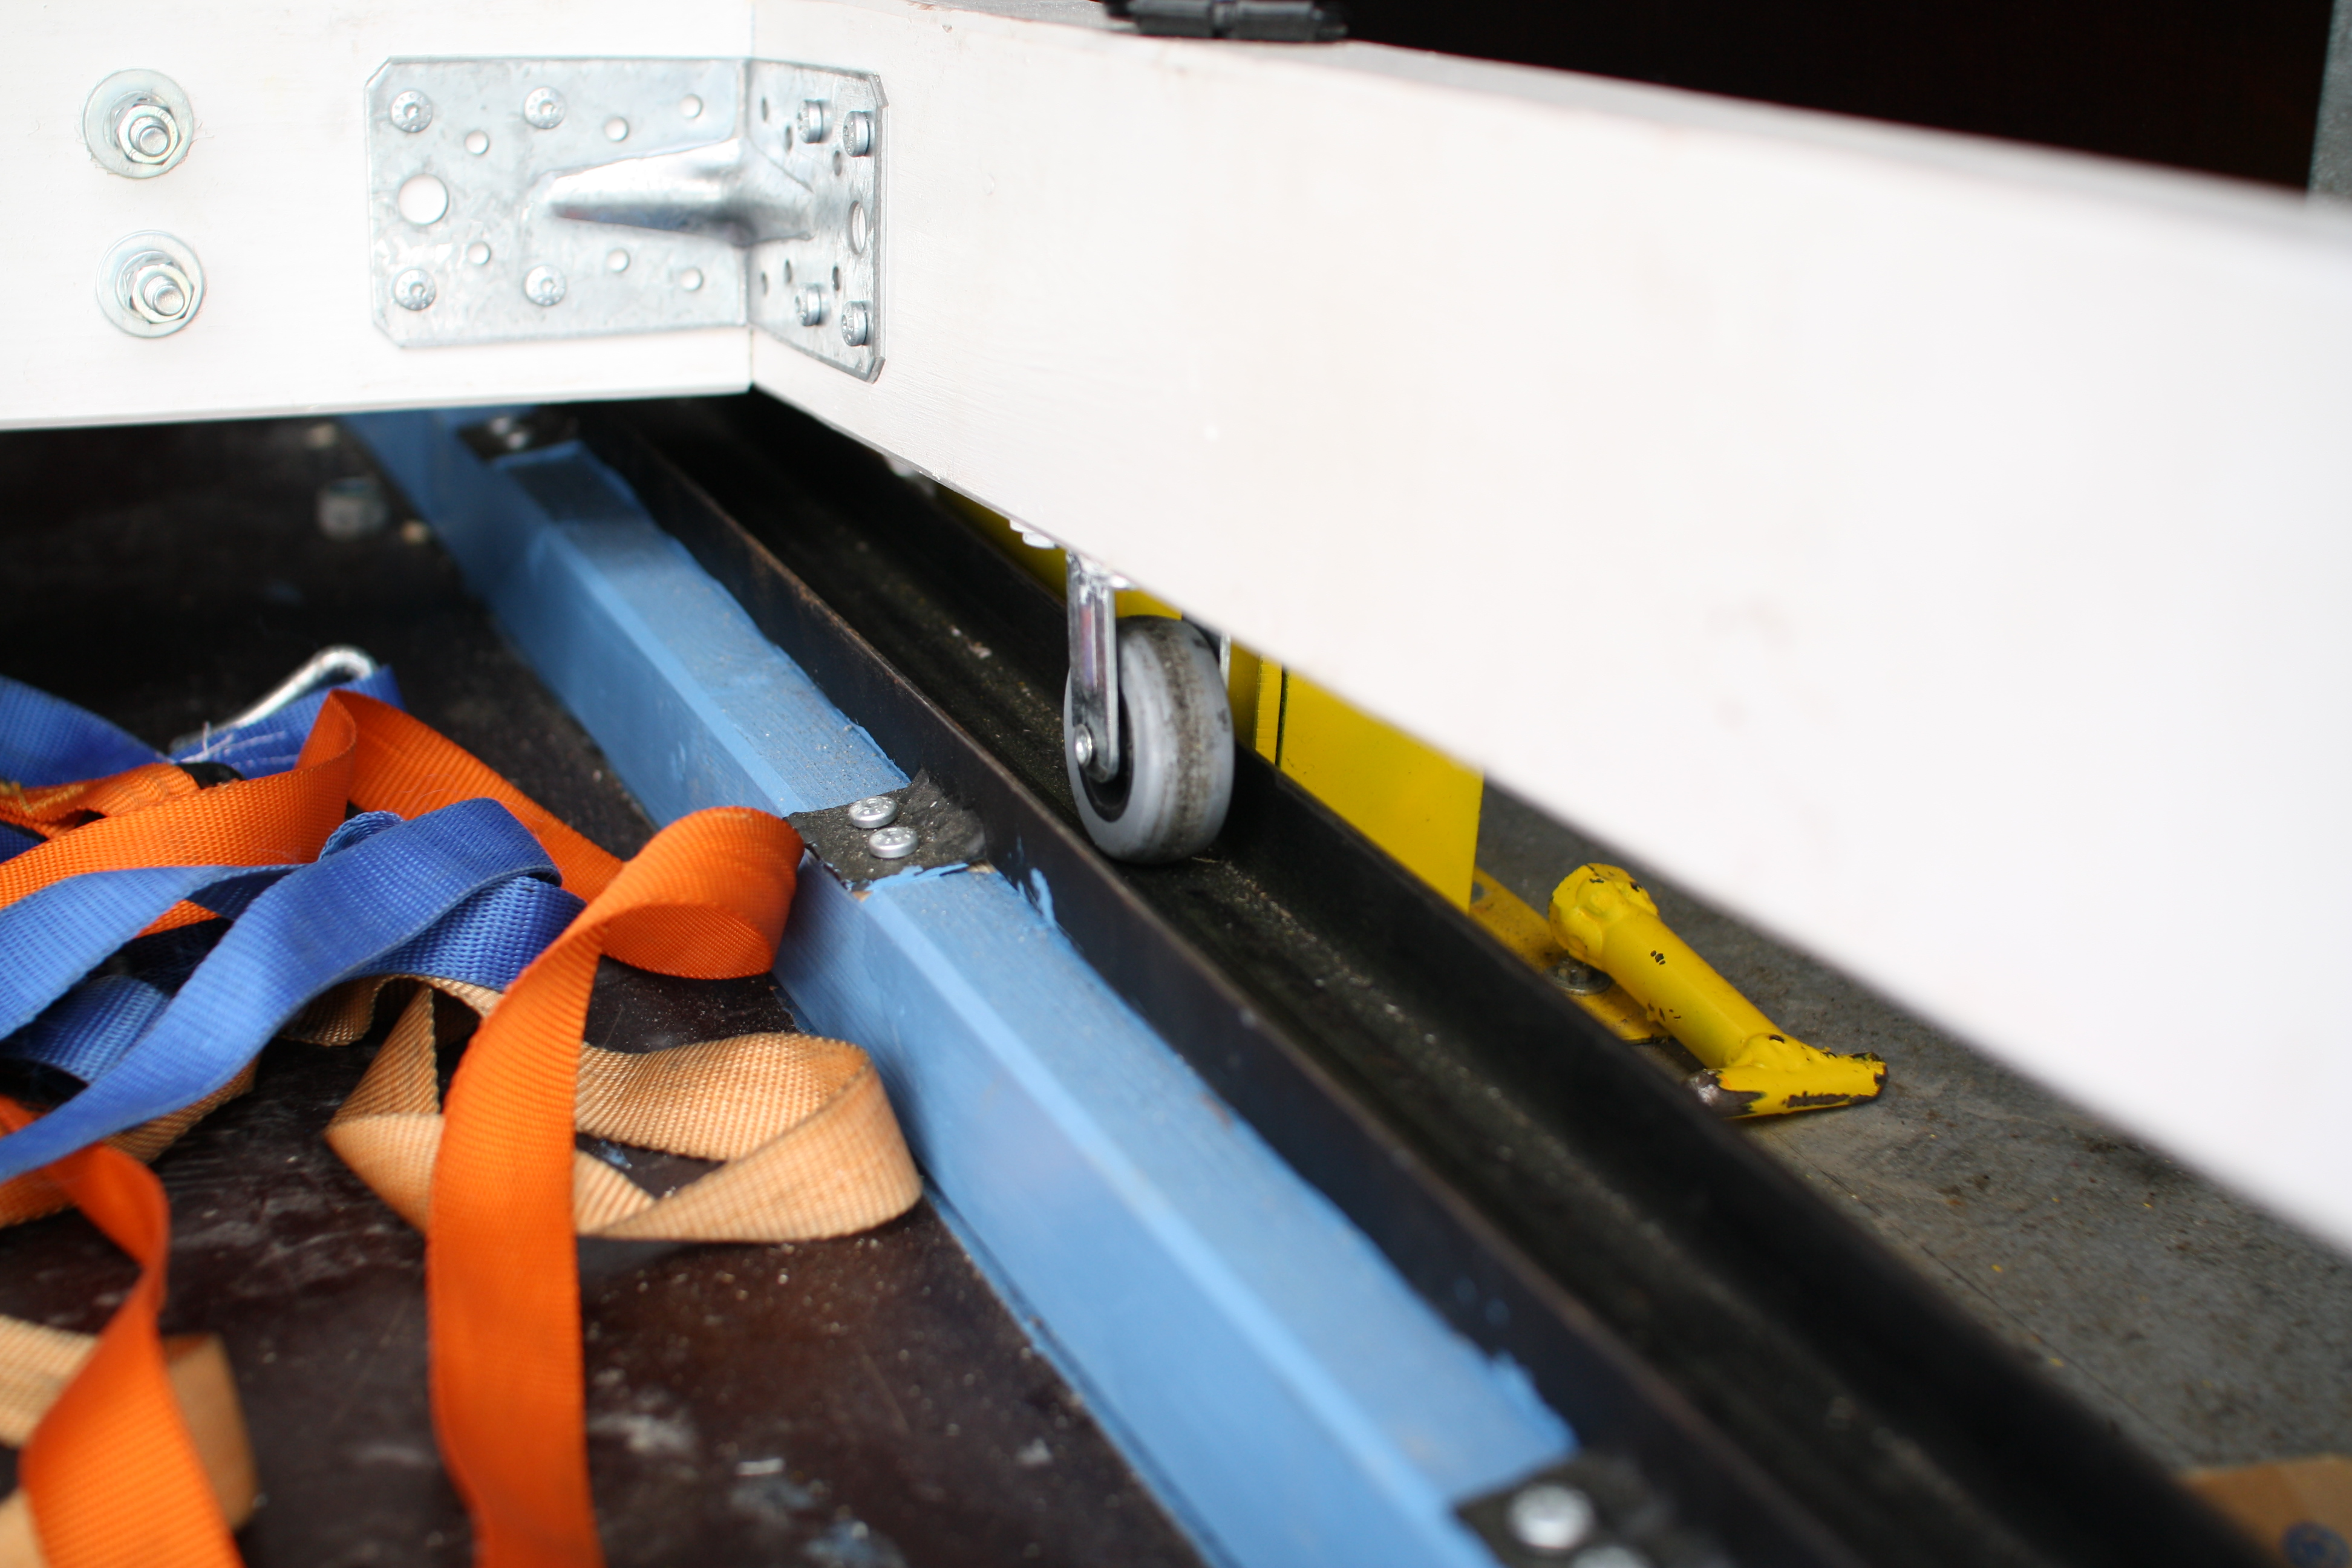
\includegraphics[width=0.5\textwidth]{images/DL3.JPG}}
\caption{Konstruksjonen}
\label{F1}
\end{figure}

Låsingen er en enkel mekanisme bestående av to låsepinner som treffer to hylser på baksiden av rammen, og to braketter der to skruer blir ført gjennom for så å bli låst med en bolt. Se Figur \ref{F2} 

\begin{figure}[h!]
\centering   
\subfloat[Fremre låsing]{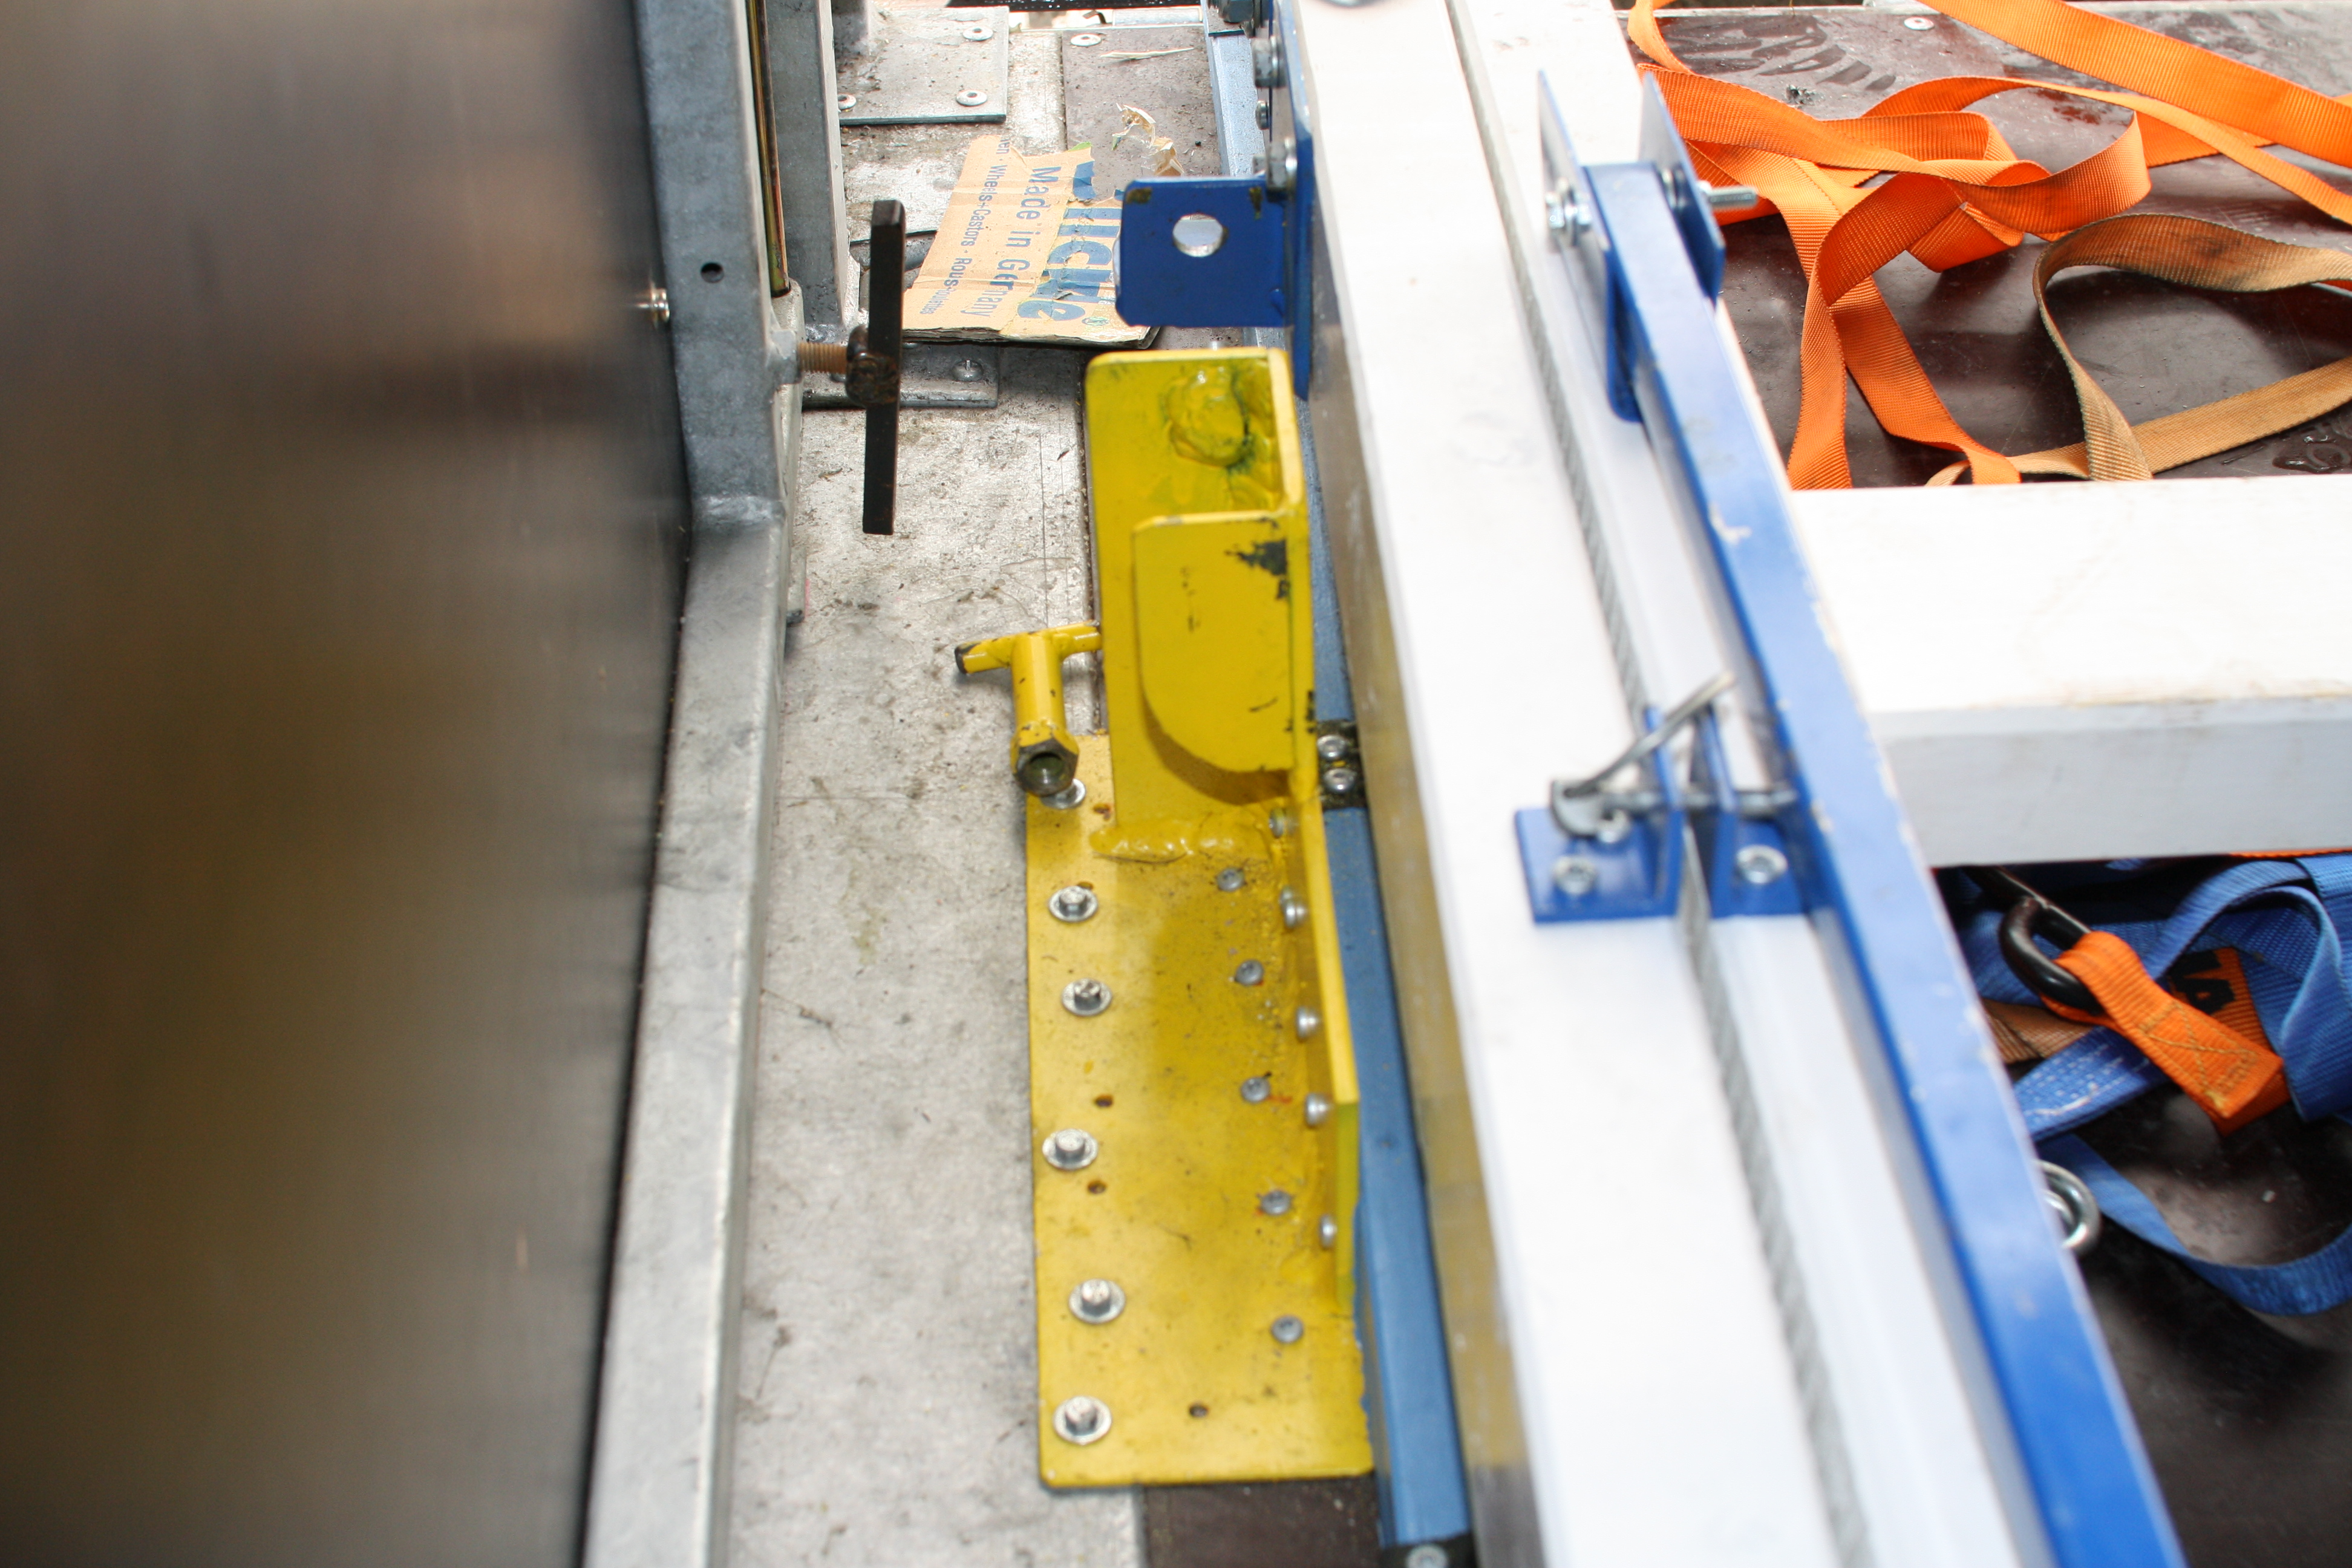
\includegraphics[width=0.5\textwidth]{images/DL5.JPG}}
\subfloat[Bakre låsing]{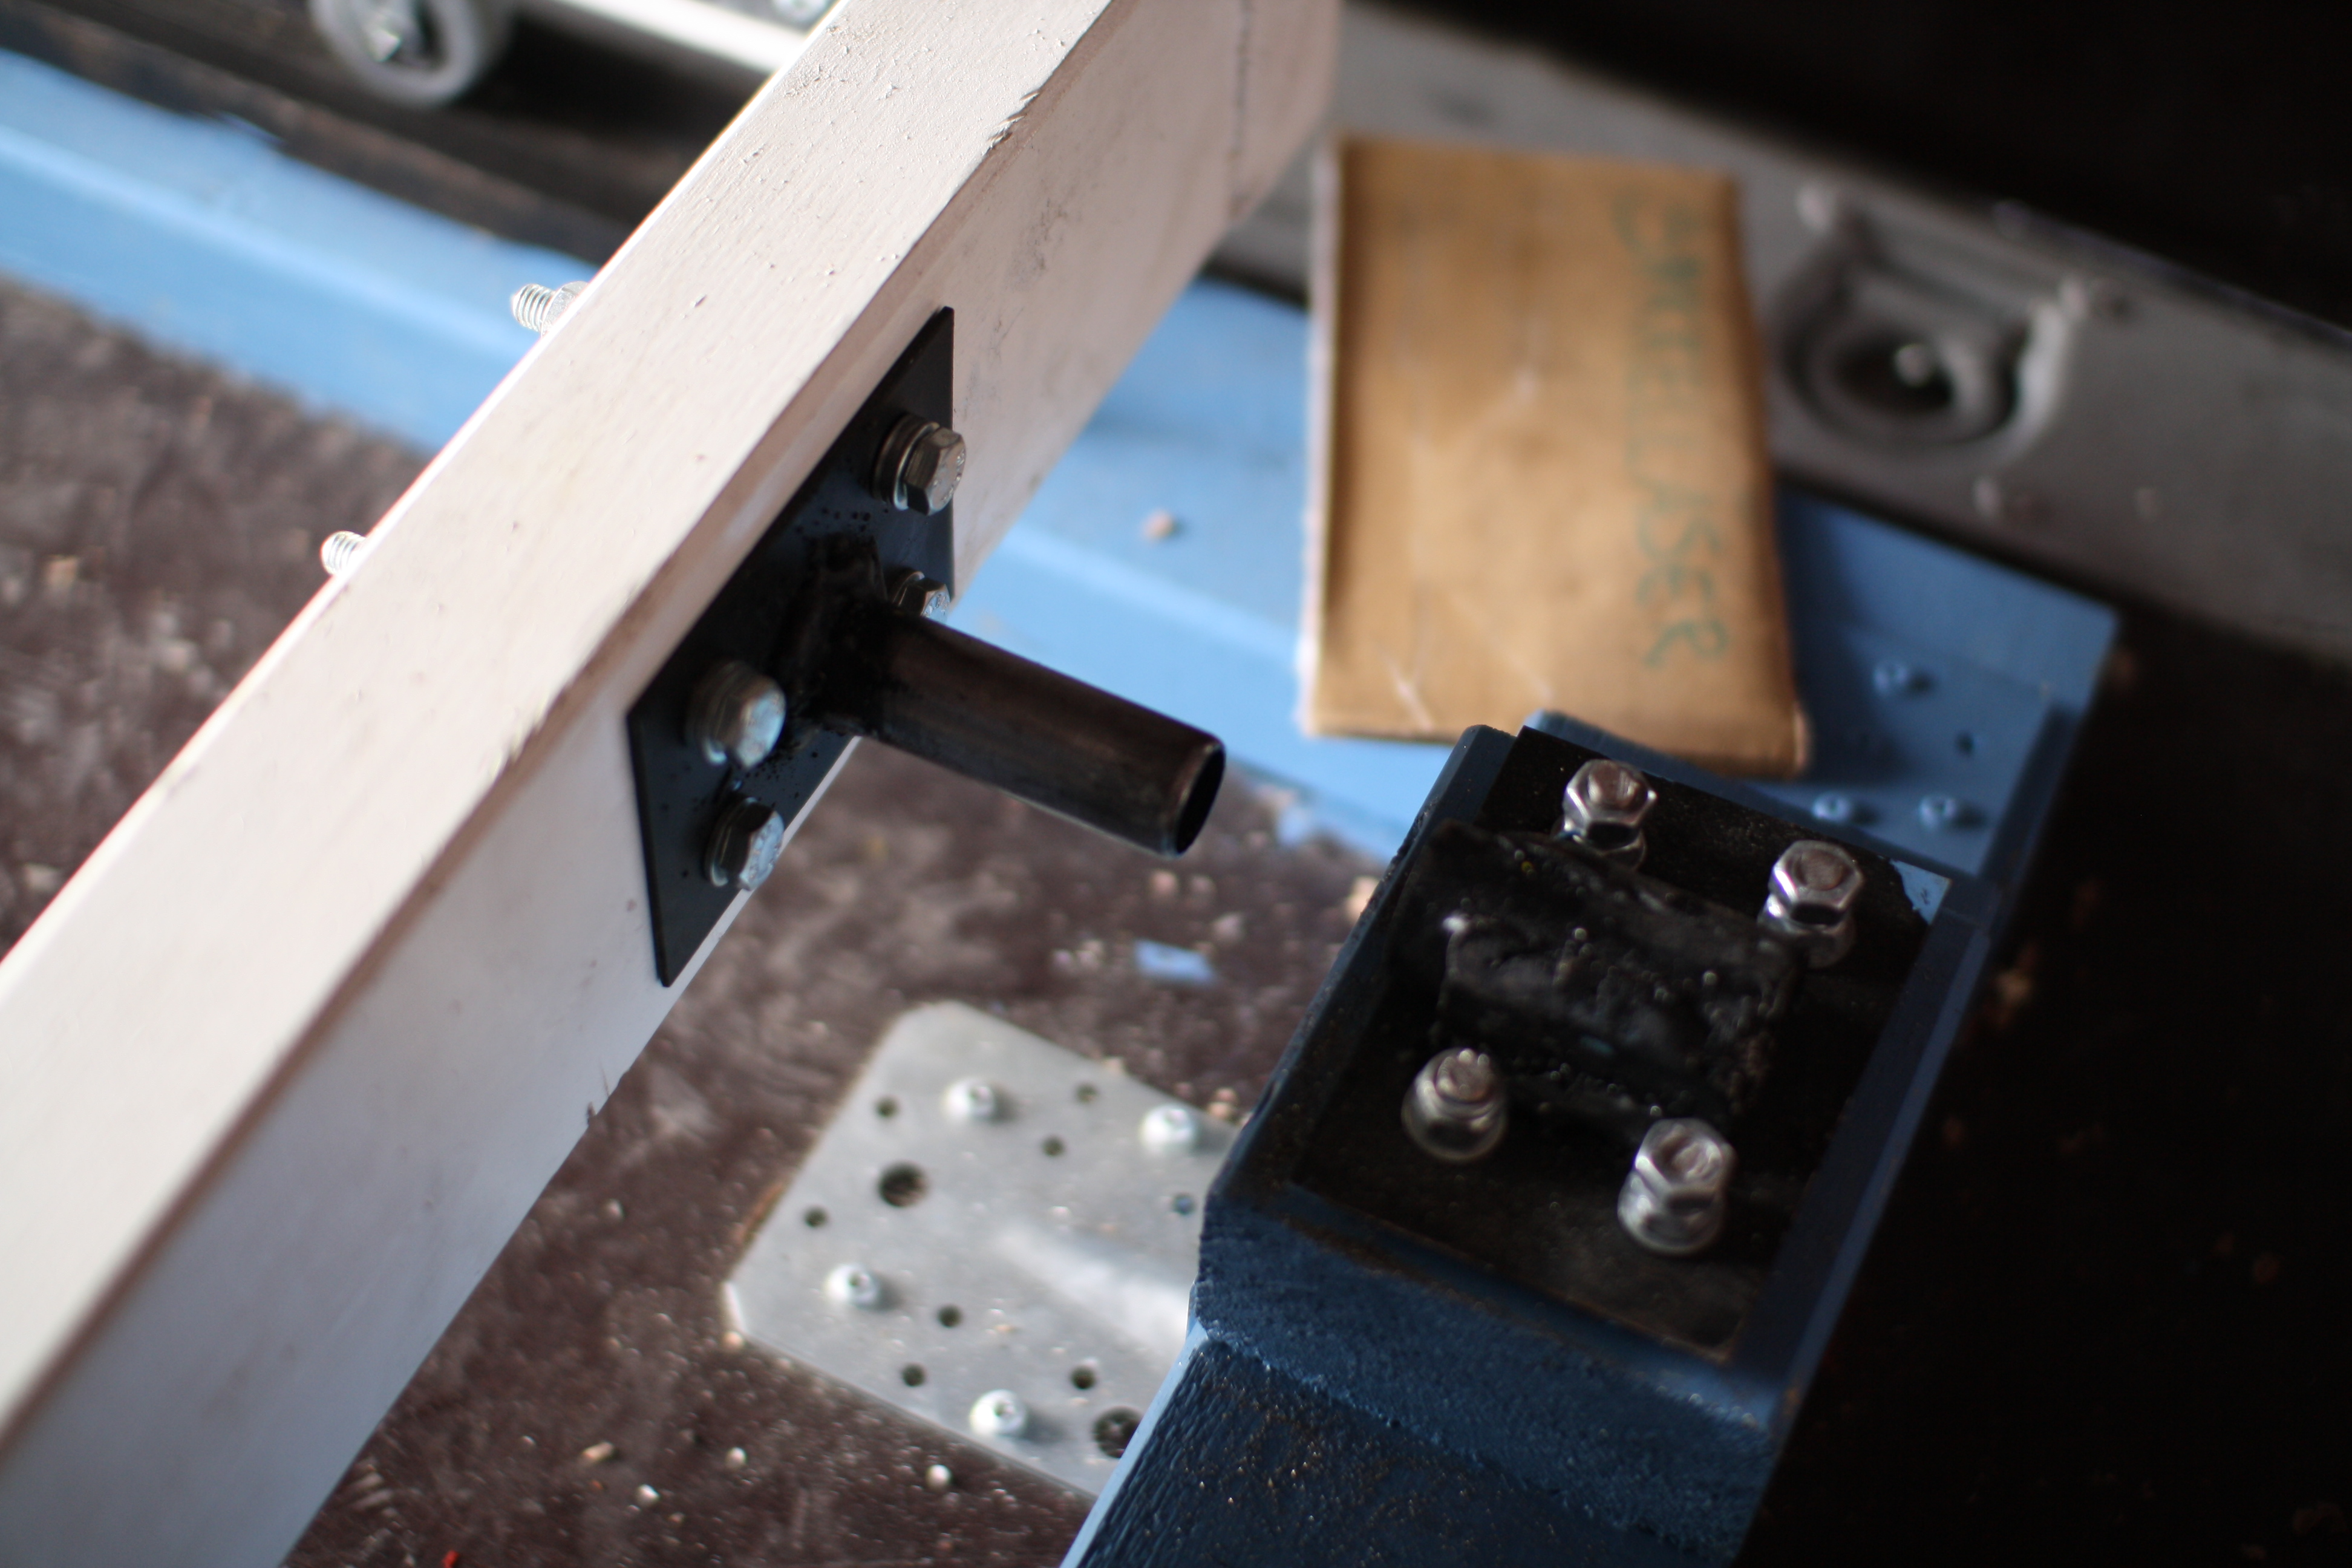
\includegraphics[width=0.5\textwidth]{images/DL4.JPG}}
\caption{Låsingen}
\label{F2}
\end{figure}

Rammen er også utstyrt med bein, slik at bilen kan stå på rammen, ute av bilen. Dette er en fordel om rammen skal brukes ved utstillinger og promoteringsoppdrag.  Se Figur \ref{F3} 

\begin{figure}[h!]
\centerline{\includegraphics[width=15cm]{images/DL2.JPG}}
\caption{Vinkelstål}
\label{F3}
\end{figure}

\subsubsection{Ulemper med dagens løsning}

En av de største ulempene med dagens løsning er at rammen bilen ikke er låst i vertikalretning når bilen skal inn og ut av henger. Dette medfører en del ekstra arbeid for de involverte og er noe som Eco maraton teamet har vert misfornøyde med.

En annen ulempe er at det er vanskelig for en person å ta ned beina mens han samtidig tar ut rammen. Dette er både et praktiskproblem men det er også problematisk rent sikkerhetsmessig. 

Det er også problematisk at puten bilen ligger på under transport er for høy, slik at det blir vanskelig å få bilen inn i hengeren. Problemet ligger i at rammen puten er festet på er for høy og at bilen må presses ned av en person samtidig som bilen blir ført inn i henger av en annen.

Hjulene på rammen er et av de største irritasjonsmomentene for de daglige brukerne. Hjulene er for små og mangler nødvendig opplagring i form av solide kulelager. Rammen blir derfor eksepsjonelt vanskelig å få ut og inn av hengeren. 

\subsubsection{Fordeler med dagens løsning}

Den store fordelen med dagens design er at bilen kan bli fraktet i henger både med og uten hjul. Dette medfører at hjulene på bilen ikke er nær bakken under transport. Slik unngås unødvendige belastninger på hjulopphenget, som i utgangspunktet ikke tåler for mye slag, eller plutselige kraftpåkjenninger. 

En annen fordel med dagens design er at det for det meste er laget i tre, dette gjør modifikasjoner relativt enkle da alt er skrudd sammen med treskruer.


